\begin{figure}[tb]
\centering
\begin{minipage}[t]{0.48\textwidth}
\centering
\textbf{(a) Recover the center}\par\smallskip
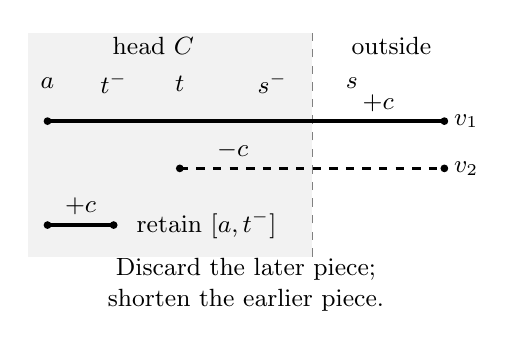
\begin{tikzpicture}[x=0.84cm,y=0.8cm,font=\small]
 \fill[black!5] (-0.3,0.25) rectangle (4,3.8);
 \draw[dashed,gray] (4,0.25)--(4,3.8);
 \node at (1.6,3.6) {head $C$};
 \node at (5.2,3.6) {outside};
 \foreach \x/\name in {0/a,1/{t^-},2/t,3.4/{s^-},4.6/s}
  {\node at (\x,3.0) {$\name$};}
 \draw[very thick] (0,2.4)--(6,2.4);
 \fill (0,2.4) circle (1.4pt); \fill (6,2.4) circle (1.4pt);
 \node[above] at (5,2.4) {$+c$};
 \node[right] at (6,2.4) {$v_1$};
 \draw[very thick,dashed] (2,1.65)--(6,1.65);
 \fill (2,1.65) circle (1.4pt); \fill (6,1.65) circle (1.4pt);
 \node[above] at (2.8,1.65) {$-c$};
 \node[right] at (6,1.65) {$v_2$};
 \draw[very thick] (0,0.75)--(1,0.75);
 \fill (0,0.75) circle (1.4pt); \fill (1,0.75) circle (1.4pt);
 \node[above] at (0.5,0.75) {$+c$};
 \node[right,align=left] at (1.2,0.75) {retain $[a,t^-]$};
 \node[align=center] at (3,-0.2) {Discard the later piece;\\shorten the earlier piece.};
\end{tikzpicture}
\end{minipage}\hfill
\begin{minipage}[t]{0.48\textwidth}
\centering
\textbf{(b) Recover one exterior piece}\par\smallskip
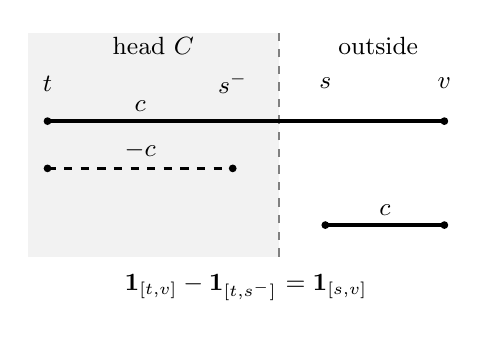
\begin{tikzpicture}[x=0.84cm,y=0.8cm,font=\small]
 \fill[black!5] (-0.3,0.25) rectangle (3.5,3.8);
 \draw[dashed,gray] (3.5,0.25)--(3.5,3.8);
 \node at (1.6,3.6) {head $C$};
 \node at (5.0,3.6) {outside};
 \foreach \x/\name in {0/t,2.8/{s^-},4.2/s,6/v}
  {\node at (\x,3.0) {$\name$};}
 \draw[very thick] (0,2.4)--(6,2.4);
 \fill (0,2.4) circle (1.4pt); \fill (6,2.4) circle (1.4pt);
 \node[above] at (1.4,2.4) {$c$};
 \draw[very thick,dashed] (0,1.65)--(2.8,1.65);
 \fill (0,1.65) circle (1.4pt); \fill (2.8,1.65) circle (1.4pt);
 \node[above] at (1.4,1.65) {$-c$};
 \draw[very thick] (4.2,0.75)--(6,0.75);
 \fill (4.2,0.75) circle (1.4pt); \fill (6,0.75) circle (1.4pt);
 \node[above] at (5.1,0.75) {$c$};
 \node[align=center] at (3,-0.2) {$\mathbf1_{[t,v]}-\mathbf1_{[t,s^-]}$
  \strut$=\mathbf1_{[s,v]}$};
\end{tikzpicture}
\end{minipage}
\caption{Segment matching in the representative case
$a\prec t\preceq s^-$, where $a$ and $t$ are the earlier and later
starts and $s$ is the first node outside the head. Each row represents
a segment; its labels through $s$ refer to the common ancestor chain.
In (a), the displayed signs are opposite coefficient signs, with
$c>0$; they are independent of the $+$ and $-$ endpoint-origin labels.
In (b), a piece from the $+$ endpoint can have either sign of $c$.
Its exterior is reproduced using at most two segments starting at $t$.
The proof also covers coincident starts, $t=s$, and roots outside $C$.}
\label{fig:segment-matching}
\end{figure}
